\documentclass{article}
\usepackage{tikz}
\usepackage{amsmath}
\begin{document}
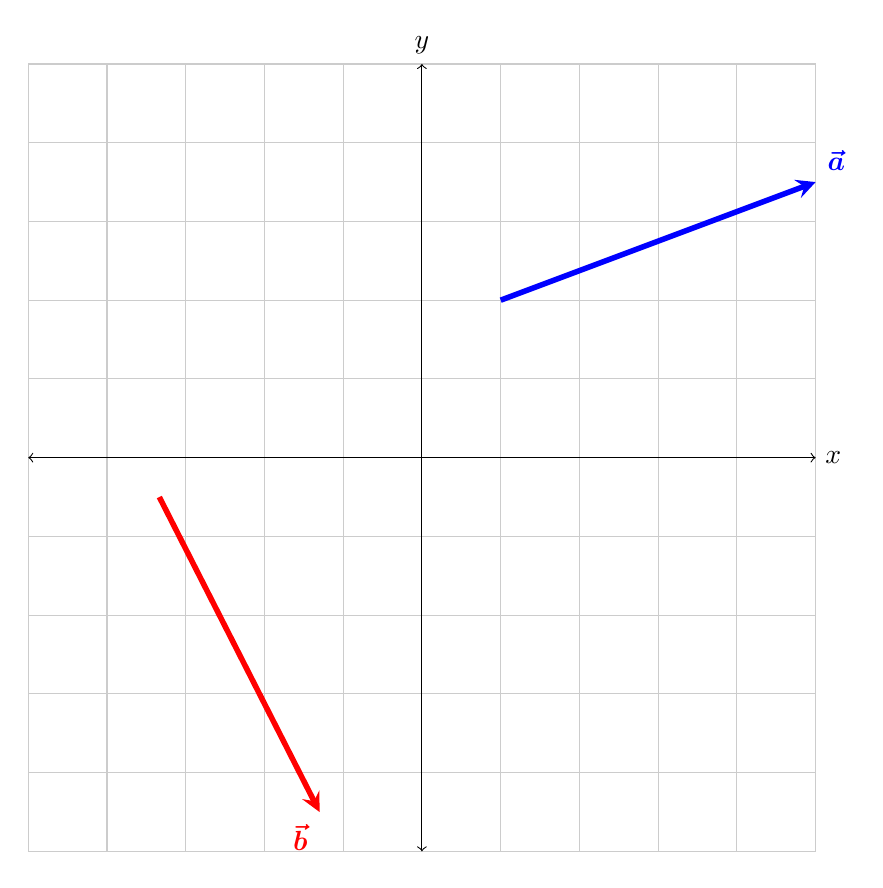
\begin{tikzpicture}
  \draw[thin,gray!40] (-5,-5) grid (5,5);
  \draw[<->] (-5,0)--(5,0) node[right]{$x$};
  \draw[<->] (0,-5)--(0,5) node[above]{$y$};
  \draw[line width=2pt,blue,-stealth](1,2)--(5,3.5) node[anchor=south west]{$\boldsymbol{\vec{a}}$};
  \draw[line width=2pt,red,-stealth](-3.335,-0.5)--(-1.3,-4.5) node[anchor=north east]{$\boldsymbol{\vec{b}}$};
\end{tikzpicture}
\end{document}